%%%%%%%%%%%%%%%%%%%%%%%%%%%%%%%%%%%%%%%%%%%%%%%%%%%%%%%%%%%%%%%%%%%%%
%% This is a (brief) model paper using the achemso class
%% The document class accepts keyval options, which should include
%% the target journal and optionally the manuscript type.
%%%%%%%%%%%%%%%%%%%%%%%%%%%%%%%%%%%%%%%%%%%%%%%%%%%%%%%%%%%%%%%%%%%%%
\documentclass[journal=jctcce,manuscript=article]{achemso}
\setkeys{acs}{articletitle=false}

%%%%%%%%%%%%%%%%%%%%%%%%%%%%%%%%%%%%%%%%%%%%%%%%%%%%%%%%%%%%%%%%%%%%%
%% Place any additional packages needed here.  Only include packages
%% which are essential, to avoid problems later. Do NOT use any
%% packages which require e-TeX (for example etoolbox): the e-TeX
%% extensions are not currently available on the ACS conversion
%% servers.
%%%%%%%%%%%%%%%%%%%%%%%%%%%%%%%%%%%%%%%%%%%%%%%%%%%%%%%%%%%%%%%%%%%%%
\usepackage[version=3]{mhchem} % Formula subscripts using \ce{}
\usepackage{chemnum}
\usepackage{multirow}
\usepackage{textgreek}
\usepackage{textcomp}
\usepackage{setspace}
\usepackage{afterpage}
\usepackage{natbib}
\usepackage[acroymn]{glossaries}
\usepackage{tabularx} % for 'tabularx' environment
\usepackage{array}

\usepackage{acro}

\acsetup{hyperref=true}

\usepackage{enumitem}

\usepackage{multicol}
\usepackage{graphicx}
\usepackage{subcaption}

% glossary
\usepackage{hyperref}


\hypersetup{
    colorlinks,
    citecolor=black,
    filecolor=black,
    linkcolor=black,
    urlcolor=black
}



%%%%%%%%%%%%%%%%%%%%%%%%%%%%%%%%%%%%%%%%%%%%%%%%%%%%%%%%%%%%%%%%%%%%%
%% If issues arise when submitting your manuscript, you may want to
%% un-comment the next line.  This provides information on the
%% version of every file you have used.
%%%%%%%%%%%%%%%%%%%%%%%%%%%%%%%%%%%%%%%%%%%%%%%%%%%%%%%%%%%%%%%%%%%%%
%%\listfiles

%%%%%%%%%%%%%%%%%%%%%%%%%%%%%%%%%%%%%%%%%%%%%%%%%%%%%%%%%%%%%%%%%%%%%
%% Place any additional macros here.  Please use \newcommand* where
%% possible, and avoid layout-changing macros (which are not used
%% when typesetting).
%%%%%%%%%%%%%%%%%%%%%%%%%%%%%%%%%%%%%%%%%%%%%%%%%%%%%%%%%%%%%%%%%%%%%
\newcommand*\mycommand[1]{\texttt{\emph{#1}}}

%%%%%%%%%%%%%%%%%%%%%%%%%%%%%%%%%%%%%%%%%%%%%%%%%%%%%%%%%%%%%%%%%%%%%
%% Meta-data block
%% ---------------
%% Each author should be given as a separate \author command.
%%
%% Corresponding authors should have an e-mail given after the author
%% name as an \email command. Phone and fax numbers can be given
%% using \phone and \fax, respectively; this information is optional.
%%
%% The affiliation of authors is given after the authors; each
%% \affiliation command applies to all preceding authors not already
%% assigned an affiliation.
%%
%% The affiliation takes an option argument for the short name.  This
%% will typically be something like "University of Somewhere".
%%
%% The \altaffiliation macro should be used for new address, etc.
%% On the other hand, \alsoaffiliation is used on a per author basis
%% when authors are associated with multiple institutions.
%%%%%%%%%%%%%%%%%%%%%%%%%%%%%%%%%%%%%%%%%%%%%%%%%%%%%%%%%%%%%%%%%%%%%
\author{Eric D. Boittier}
\email{eric.boittier@uqconnect.edu.au}
\affiliation[UQ]{The University of Queendland, St Lucia, Queensland, Australia}

\author{\linebreak Supervisors: A/Professor Vito Ferro}
\affiliation[UQ]{The University of Queendland, St Lucia, Queensland, Australia}

\author{Dr Neha Gandhi}
\affiliation[QUT]{Queensland University of Technology, Gardens Point, Queensland, Australia}


%%%%%%%%%%%%%%%%%%%%%%%%%%%%%%%%%%%%%%%%%%%%%%%%%%%%%%%%%%%%%%%%%%%%%
%% The document title should be given as usual. Some journals require
%% a running title from the author: this should be supplied as an
%% optional argument to \title.
%%%%%%%%%%%%%%%%%%%%%%%%%%%%%%%%%%%%%%%%%%%%%%%%%%%%%%%%%%%%%%%%%%%%%
\title[Honours]
  {Parameterisation of ``VinaCarb" for improved docking of heparin/heparan sulfate  \linebreak \large Research Proposal}

%%%%%%%%%%%%%%%%%%%%%%%%%%%%%%%%%%%%%%%%%%%%%%%%%%%%%%%%%%%%%%%%%%%%%
%% Some journals require a list of abbreviations or keywords to be
%% supplied. These should be set up here, and will be printed after
%% the title and author information, if needed.
%%%%%%%%%%%%%%%%%%%%%%%%%%%%%%%%%%%%%%%%%%%%%%%%%%%%%%%%%%%%%%%%%%%%%
\abbreviations{IR,NMR,UV}
\keywords{American Chemical Society}

\DeclareAcronym{Ido}{
    short = Ido ,
    long = {\small L}-iduronic acid
}

\DeclareAcronym{Glc}{
    short = Glc ,
    long = {\small D}-glucose
}

\DeclareAcronym{Gal}{
    short = Gal ,
    long = {\small D}-galactose
}

\DeclareAcronym{DFT}{
    short = DFT ,
    long = density functional theory
}

\DeclareAcronym{GlcN}{
    short = Ido ,
    long = {\small D}-glucosamine
}

\DeclareAcronym{GalA}{
    short = GalA ,
    long = {\small D}-galacturonic acid
}

\DeclareAcronym{GlcA}{
    short = GlcA ,
    long = {\small D}-glucuronic acid
}

\DeclareAcronym{GalN}{
    short = GalN ,
    long = {\small D}-galactosamine
}

\DeclareAcronym{GlcNAc}{
    short = GlcNAc ,
    long = {\small D}-N-acetylglucosamine
}

\DeclareAcronym{GalNAc}{
    short = GalNAc ,
    long = {\small D}-N-acetylgalactosamine
}

\DeclareAcronym{Ido}{
    short = Ido ,
    long = {\small L}-iduronic acid
}


\DeclareAcronym{PG}{
    short = PG ,
    long = proteoglycan
}

\DeclareAcronym{ECM}{
    short = ECM ,
    long = extracellular matrix
}

\DeclareAcronym{GAG}{
    short = GAG ,
    long = glycosaminoglycan
}

\DeclareAcronym{Hep}{
    short = Hep ,
    long = heparin
}
\DeclareAcronym{HS}{
    short = HS ,
    long = heparan sulfate
}
\DeclareAcronym{HA}{
    short = HA ,
    long = hyaluronic acid
}
\DeclareAcronym{CS}{
    short = CS,
    long = chondroitin sulfate
}
\DeclareAcronym{KS}{
    short = KS,
    long = keteran sulfate
}
\DeclareAcronym{DS}{
    short = DS,
    long = dermatin sulfate
}


\DeclareAcronym{DoS}{
    short = DoS,
    long = degree of sulfation
}

\DeclareAcronym{SNFG}{
    short = SNFG, 
    long = structural nomenclature for glycans
}


\DeclareAcronym{APP}{
    short = APP,
    long = amyloid precursor protein
}
\DeclareAcronym{Al}{
    short = APP,
    long = amyloid precursor protein
}
\DeclareAcronym{QM}{
    short = QM,
    long = quantum mechanics
}
\DeclareAcronym{md}{
    short = MD,
    long = molecular dynamics
}


\DeclareAcronym{FGF1}{
    short = FGF1,
    long = fibroblast growth factor 1
}
\DeclareAcronym{FGF2}{
    short = FGF2,
    long = fibroblast growth factor 2
}
\DeclareAcronym{FGF}{
    short = FGF,
    long = fibroblast growth factor 
}
\DeclareAcronym{AT3}{
    short = ATIII,
    long = \textalpha-antithrombin III
}

\DeclareAcronym{RMSD}{
    short = RMSD,
    long = root mean square deviation
}
\DeclareAcronym{PRMSD}{
    short = PRMSD,
    long = pose root mean square deviation
}

\DeclareAcronym{RBD}{
    short = RBD,
    long = rigid body docking
}




\begin{document}


%%%%%%%%%%%%%%%%%%%%%%%%%%%%%%%%%%%%%%%%%%%%%%%%%%%%%%%%%%%%%%%%%%%%%
%% The manuscript does not need to include \maketitle, which is
%% executed automatically.  The document should begin with an
%% abstract, if appropriate.  If one is given and should not be, the
%% contents will be gobbled.
%%%%%%%%%%%%%%%%%%%%%%%%%%%%%%%%%%%%%%%%%%%%%%%%%%%%%%%%%%%%%%%%%%%%%
{\setstretch{1.5} 
\renewcommand{\contentsname}{Table of Contents}

\newpage
\tableofcontents
\newpage
\listoffigures
\listoftables
\begin{multicols}{2}
{\setstretch{1}
\printacronyms[name={Abbreviations}, list-style={table}]
}
\end{multicols}

%%%%%%%%%%%%%%%%%%%%%%%%%%%%%%%%%%%%%%%%%%%%%%%%%%%%%%%%%%%%%%%%%%%%%
%% Start the main part of the manuscript here.
%%%%%%%%%%%%%%%%%%%%%%%%%%%%%%%%%%%%%%%%%%%%%%%%%%%%%%%%%%%%%%%%%%%%%
\pagebreak
\section{Background}

\subsection{Heparin and heparan sulfate}
Carbohydrates have been likened to the third molecule of life after aminoacids and nucleic acids.
\Acp{GAG} are a family of linear oligosaccharides comprised of repeating disaccharide units whose family members, \ac{Hep}/\ac{HS} (shown in Table \ref{tab:my_label}), posses some of the highest negative charge density found in nature \cite{Gandhi2008TheProteins,Swarup2013SugarNeurons}. \Acp{GAG} are present in the extracellular matrix \ac{ECM} of all animal cells, found on the surface and in solution.

\subsubsection{Structure}
\acp{GAG} are comprised of repeating units of uronic acid residues (\ac{GlcA} or \ac{Ido}) and amino sugar residues (\ac{GalN} or \ac{GlcN}). All \acp{GAG}, apart from \ac{HA}, exhibit various sulfation patterns and \acf{DoS}. The amino sugar can be sulphated at C4, C6, the unsubstituted nitrogen or C3 (rare), and the uronic acid residue can be substituted at a variety of positions -- leading to \textgreater1000 possible substitution patterns for a simple octasaccharide.\cite{Gandhi2008TheProteins, SoaresdaCosta2017SulfationDisorders}
At physiological pH, all carboxylic acid and sulphate groups are deprotonated. 
GAG sulfation patterns have been likened to the “sulfation code” as there is believed to be high specificity in relation to function.\cite{Habuchi2004SulfationCode, Gama2006SulfationActivity}

\afterpage{
\begin{table}[H]
\begin{tabular}{p{5em}p{14em}p{17em}} \hline \hline
    GAG & Major repeating units & Features \tabularnewline \hline \hline
    
    \vspace{0.25mm} Heparin (Hep) & 
    \vspace{0.01mm}\hspace{5mm}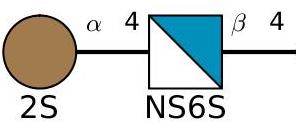
\includegraphics[width=3.5cm]{structures/HepSNFG.jpg}
    
    \hspace{5mm}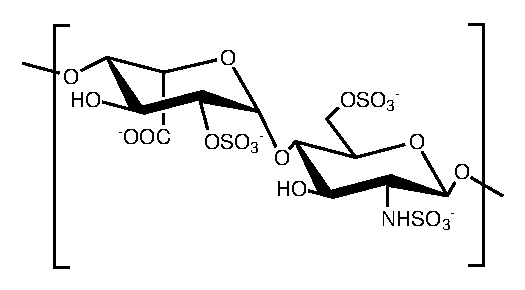
\includegraphics[width=4cm]{structures/heparin.eps}
    
    \hspace{-1mm}{\small L}-Ido2S-\textalpha(1\textrightarrow4)-{\small D}-GlcNS-\textalpha(1-4) \vspace{1mm} 
    &\vspace{-1mm} \textbf{Possible sulfation:} \newline \textbf{GlcNS:} 3S, 6S. \vspace{1mm}\hline\vspace{1mm} \textbf{\Ac{DoS}:} 1.8 -- 2.6\cite{SoaresdaCosta2017SulfationDisorders}/2.7\cite{Capila2002Heparin-proteinInteractions.}
    % \vspace{1mm}\hline\vspace{1mm} \newline
    \tabularnewline
    
    \hline
    \vspace{2mm}Heparan sulfate (HS) & { \vspace{0.1mm}
    \hspace{5mm}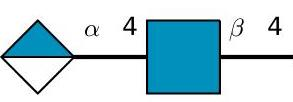
\includegraphics[width=3.5cm]{structures/HSSNFG.jpg}
    
    \hspace{5mm}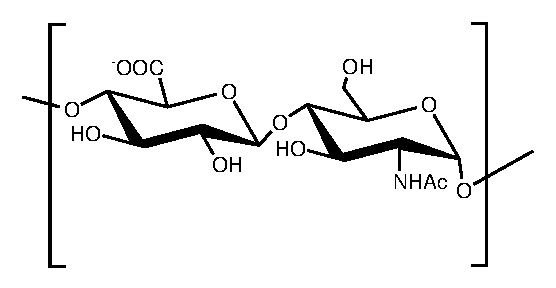
\includegraphics[width=4cm]{structures/heparan.eps}}
    
    \hspace{-4mm}{\small D}-GlcA-\textalpha(1\textrightarrow4)-{\small D}-GlcNAc-\textbeta(1-4) \vspace{0mm} \newline
    & \vspace{-0.5mm}\textbf{Possible sulfation:} \newline \vspace{0.5mm}\textbf{GlcA:} 2S, \textbf{GlcNS:} 3S, 6S.
    \vspace{1mm}\hline\vspace{1mm}\textbf{\Ac{DoS}:} 0.8 -- 1.8\cite{SoaresdaCosta2017SulfationDisorders}
    % \vspace{1mm}\hline\vspace{1mm} \newline
    \tabularnewline
    \hline
    \hline

\end{tabular}

    \caption{The structure and features of heparin and heparan sulfate, including \ac{DoS} and \acf{SNFG}\cite{Ferguson2009EssentialsEdition} representation.}
    \label{tab:my_label}
    
\end{table}
}

\subsubsection{Protein interactions and cell function}
\acp{GAG} bind to distinct attachment receptors on proteins such as chemokines, cytokines, growth factors, morphogens, enzymes and adhesion molecules\cite{Murphy2007StructuralHeparin, Iozzo2001HeparanArena, Kreuger2006InteractionsSpecificity, Kowitsch2018MedicalReview}. Carbohydrates form hydrogen bonds with side chain residues of polar planar amino acid residues (ASN, ASP, GLY, GLN, ARG and HIS)\cite{Malik2007SequenceNetwork}.
These hydrogen bonds can be cooperative hydrogen bonds, bidentate hydrogen bonds or hydrogen bond networks and facilitate low energy conformations of the polysaccharide.\cite{Quiocho1989Protein-carbohydrateFeatures} 

\ac{HS} and other \acp{GAG} can interact with AB peptides and enhance the shift of AB42 peptides to the \textbeta-sheet confirmation.

\ac{HS} and \ac{Hep} are key to the regulation of Alzheimer's  \textbeta-secretase (BACE1), as they bind to BACE-1 and inhibit cleavage of \ac{APP} and aggregate into amyloid plaques involved with the overall progression of the disease.\cite{Swarup2013SugarNeurons,Scholefield2003HeparanBeta-secretase.}

GAGs in solution can inhibit proteins that target specific GAG sequences on the surface of \acp{PG}. For example, a heparin pentasaccharide interacts with certain binding pockets on \ac{FGF} blocking interactions with proteins associated with proteolysis, which proliferates the \acp{FGF}, causing morphological changes to the cell\cite{SoaresdaCosta2017SulfationDisorders}. 
\\
GAG sulfation creates specific microenvironments at the \ac{ECM}, which serves to direct the permeation of small cations, the proliferation of stem cells and the regulation of neuronal development in humans, amongst other processes. 



\pagebreak
\subsection{Computational methods and carbohydrates}

`Big O'  notation, $\mathcal{O}(f(n))$, is a concept in computer science that relates the size of a task to the time taken to complete the task using a given algorithm. A task of $\mathcal{O}(n^{2})$ implies a quadratic relationship between the size of the task and the time taken to complete it.

\subsubsection{Quantum mechanics}
\Ac{QM} is ...
\Ac{QM} has the ability to give reliable results, such as energies and geometries, that can be used to give approximations using `cheaper' computational methods (such as force fields or energy functions for docking experiments). 

GLYCAM06, an Amber forcefield that provides the basis of energy calculations in VinaCarb, was parameterized using the HF/6-31G* level of theory for geometry optimization and B3LYP/6-3111G(2d,2p) for single point energy calculations\cite{Kirschner2008GLYCAM06:Carbohydrates}. 
During geometry optimization, diffuse functions were added to anionic molecules; however, this approach was not taken during the calculation of single point energies. It is likely therefore, that free energies may be underestimated for anionic compounds. Since solvation effects are key considered key to understanding the thermodynamics of carbohydrates, especially highly charged sugars such as \acp{GAG}, since the parameterization of GLYCAM06 neglected the use of appropriate implicit solvents, such as water, it would be prudent to consider this error when evaluating the accuracy of this model. 

In terms of how this functional/basis set combination performs to higher levels of theory, there has been some effort made to benchmark these details when studying these molecules with \ac{DFT}. Although many examples of its use exist in the literature, B3LYP has shown to perform poorly when compared to high level \textit{ab initio} calculations, such as MP2/aug-cc-pVTZ and CCSD(T). CCSD(T) methods scale $\mathcal{O}(n^{7})$ in terms of system size, making high quality calculations of disaccharides prohibitively expensive with current technology. 

GLYCAM06 shows an unsatisfying performance in the entire energy window

A bench marking study involving 

M06-L performed 

\subsubsection{Molecular dynamics}
\Ac{md}

\subsubsection{Docking}

\subsubsection{Statistical methods}

The distribution of amino acid residues at carbohydrate binding sites suggests

\subsection{Current advances in GAG/carbohydrate docking}

\subsubsection{Cluspro: heparin site mapping (2014)}

The Cluspro server is an online protein--protein docking package which was adapted in 2014 to include a tool used for \ac{Hep}/\ac{HS} site mapping tool.\cite{Comeau2007ClusPro:Server, Mottarella2014DockingProteins,Kozakov2017TheDocking.} 
Cluspro performs three main computational procedures: \ac{RBD}, \ac{RMSD} clustering and refinement using an energy minimization function.\cite{Kozakov2017TheDocking.} 


\subsubsection{VinaCarb (AutoDock Vina) (2016)}
\ac{RMSD}
\ac{PRMSD}

\subsubsection{GAG--Dock (DarwinDock/GenDock) (2017)}
The ``GAG-Dock" method reported by
\citeauthor{Griffith2017PredictingGrowth}\cite{Griffith2017PredictingGrowth} was developed using DarwinDock and GenDock to model GAG--protein interactions. This method accurately predicted \ac{Hep} binding poses within 0.70 - 1.51 \r{A} \ac{RMSD} of the crystal structures (\ac{FGF1}, \ac{FGF2}, and \ac{AT3}. The authors also investigated the specificity of protein binding, through in silico mutations, to favor a particular GAG sulfation pattern. 
To establish the available space for a ligand to dock, a modified version of the sphgen program\cite{Moustakas2006Development5} was used. Sphgen generates concentric spheres that combine to form a curve topology which is used to model the surface of the protein. 
Sphgen can also be used to analysing clustering of docked ligands.\cite{Hendrix1998SurfaceDocking.}
To model \ac{GAG} binding to flat surface, the available space for ligands to bing to flat protein surfaces was increased. In this modification, the “dotlim” parameter in sphgen was altered. The default ``dotlim" value, zero, prevents generation of large spheres with close surface contacts.\cite{Hendrix1998SurfaceDocking.} For \acp{GAG} ``dotlim" parameter was decreased to - 0.9, which allowed for spheres to be generated for flat surfaces.\cite{Griffith2017PredictingGrowth} To prevent sampling from pockets inside the protein that would be inaccessible to \asp{GAG}, a two sphere surfaces are generated by using the normal probe radius the normal 1.4 \r{A} and a larger radius of 2.8 \r{A}. The intersection of these surfaces is taken to generate spheres on the protein surface without sampling from too close to, or outside of, the surface.\cite{Griffith2017PredictingGrowth} 

\subsection{Current challenges in glycosaminoglycan docking}

\pagebreak
\section{Aims}

\section{Methods}


}
\newpage
{\setstretch{0}
\bibliography{mendeley_v2}
}
\newpage
\section{Appendix}
\end{document}

